% !TEX root = ../../main.tex
% !TEX spellcheck = en_GB

\section{Modelling}
\label{sec:PureSineModelling}

The Matlab code for pitch shifting an input sine of \SI{470}{\hertz} is shown in \cref{app:matlabmodel}. It is primarily based on the description from Matlab \cite{MatlabIF} and the open source implementation in the Octave Signal package \cite{OctaveHilbert}.

\Cref{code:matlabmodel} shows pseudo code describing the Matlab model.
The blockSize is set, and a Hamming window is generated.
The window can be used for each block and it is only necessary to generate it once.
The phase starts at zero, but is updated after each loop, allowing for the next block to start with the correct phase shift.
The loop loads the samples, applies the window, finds the frequency, finds the closest C-major frequency, generates a sine at the correct frequency and phase and updates the phase.
Finding the frequency is done by hilbert transforming the input signal, determining the phase, unwrapping the phase and then calculating the derivative of the phase.
The derivative of the phase is the frequency.

\begin{listing}
	\begin{minted}[linenos, breaklines, bgcolor=lightgray]{matlab}
blockSize = 512;
h = hammingWindow(blockSize);
phase = 0;

while(1)
	y = load(blockSize);
	yh = h .* y;
	freqIn = findIF(yh);
	newFreq = pianoFreq(freqIn);
	[out, phase] = genSine(blockSize, newFreq);
	\end{minted}
	\caption{Pseudo code for the Matlab model.}
	\label{code:matlabmodel}
\end{listing}

\begin{figure}
	\centering
	\begin{subfigure}[t]{.5\textwidth}
		\centering
		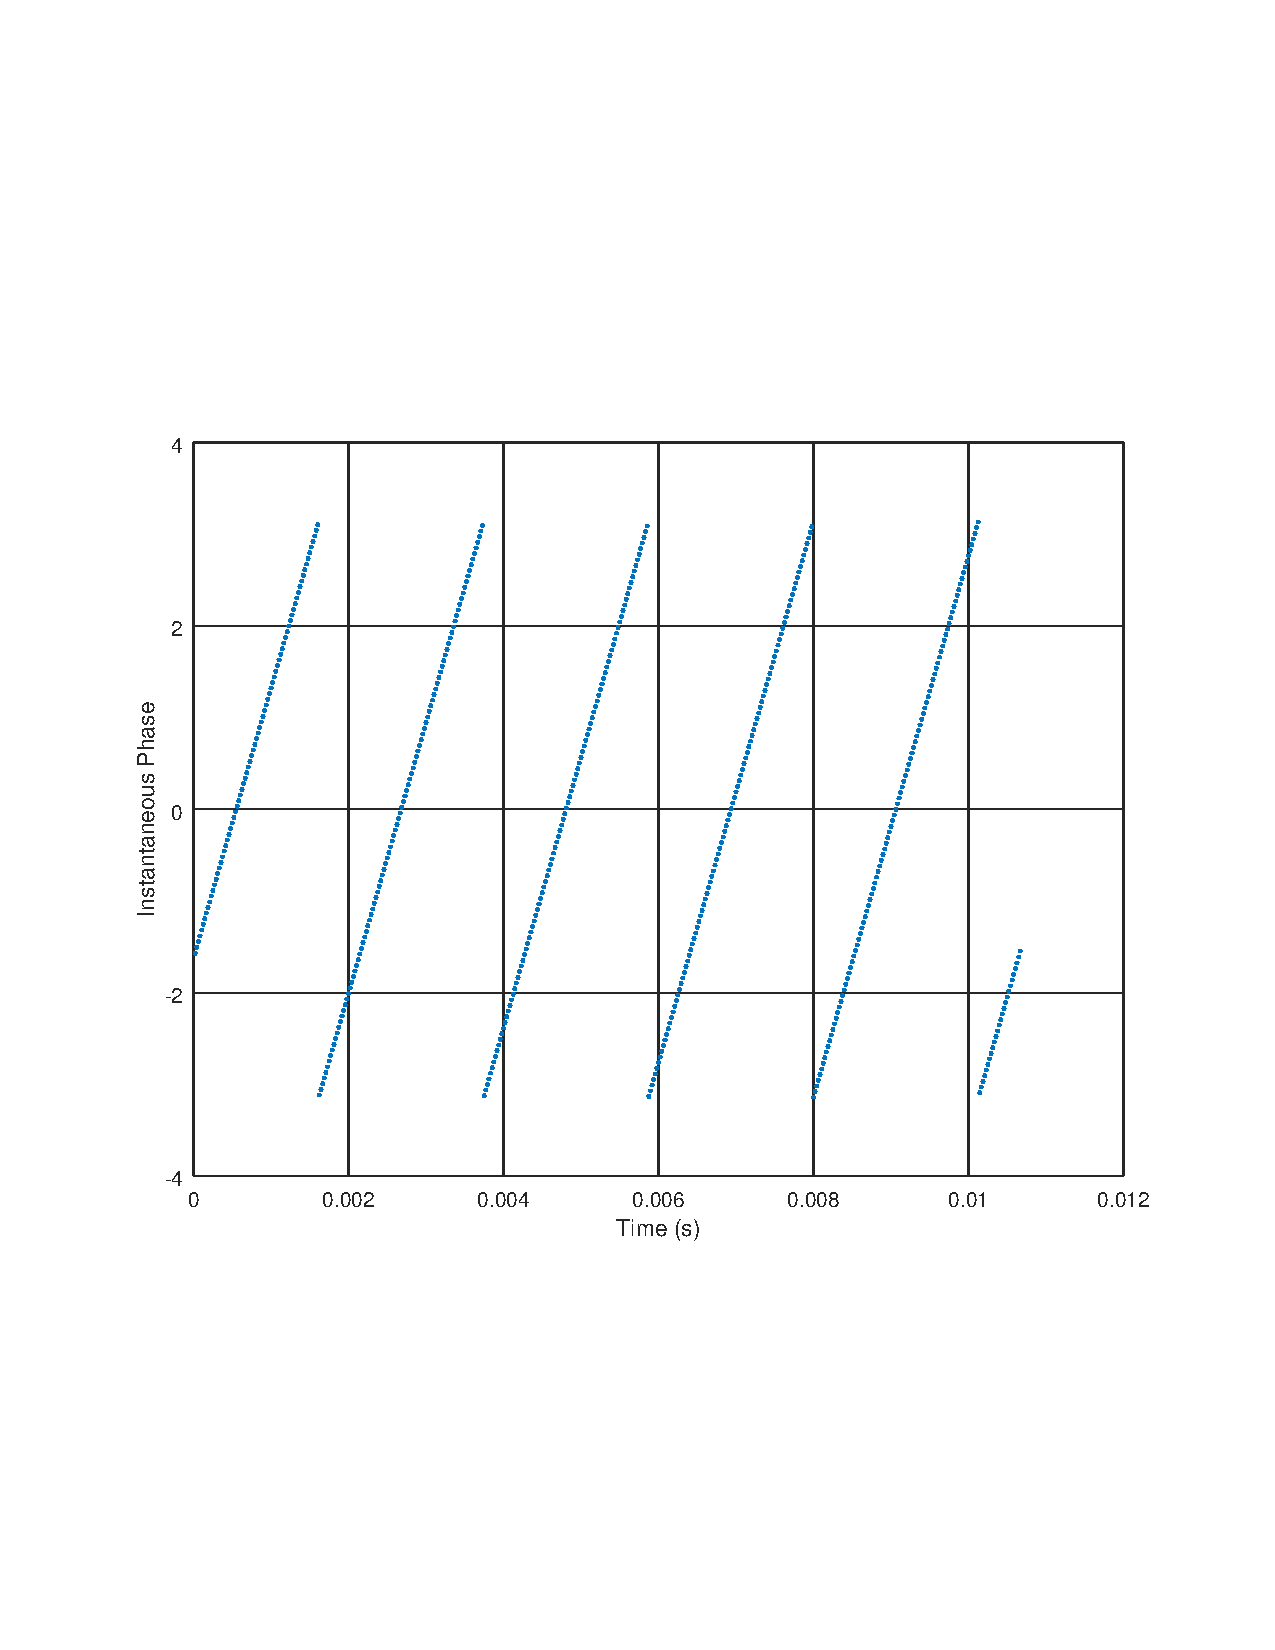
\includegraphics[width=.9\linewidth, clip, trim={2cm 7cm 2cm 7cm}]{gfx/Modelling/IFIP.pdf}
		\caption{Instantaneous Phase.}
		\label{fig:sub1}
	\end{subfigure}%
	\begin{subfigure}[t]{.5\textwidth}
		\centering
		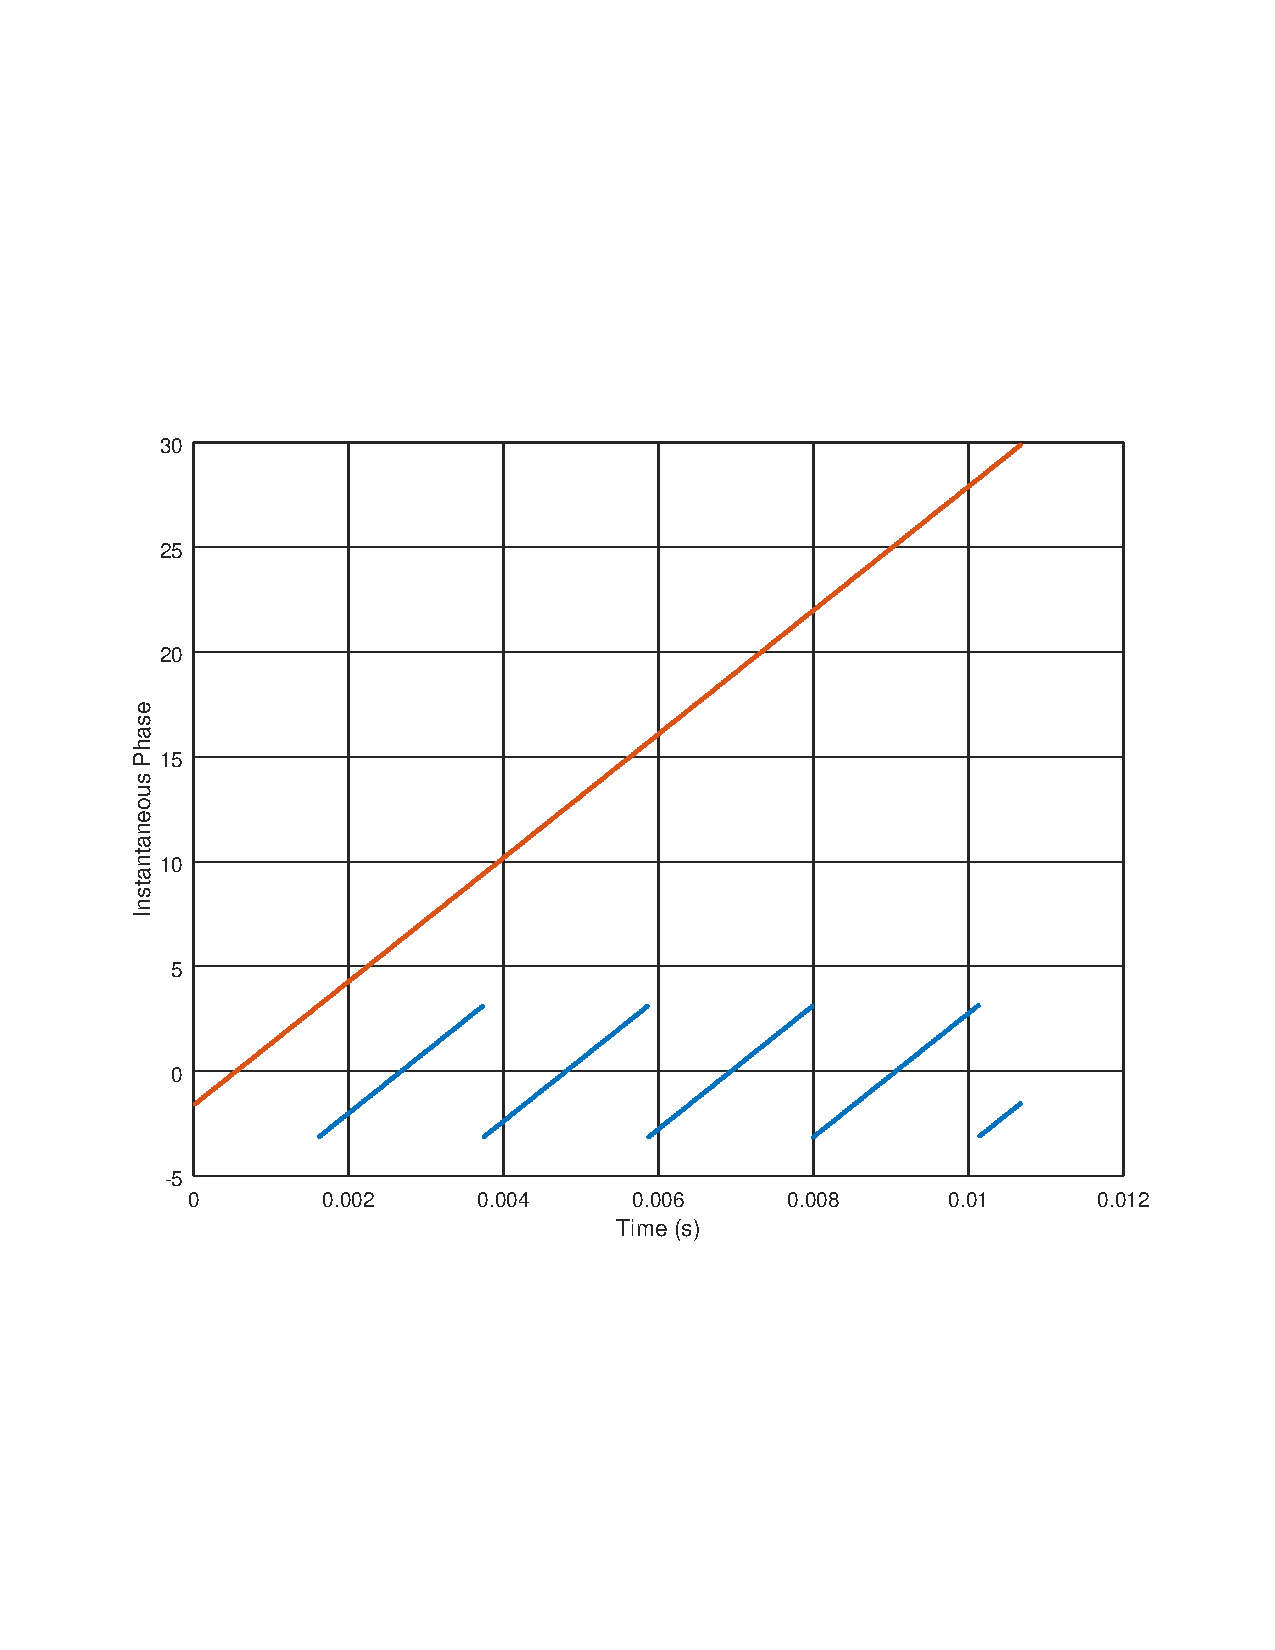
\includegraphics[width=.9\linewidth, clip, trim={2cm 7cm 2cm 7cm}]{gfx/Modelling/IFunwrap.pdf}
		\caption{Wrapping Instantaneous Phase (blue), and unwrapped Instantaneous Phase (red).}
		\label{fig:sub2}
	\end{subfigure} \\
	\begin{subfigure}[t]{.5\textwidth}
		\centering
		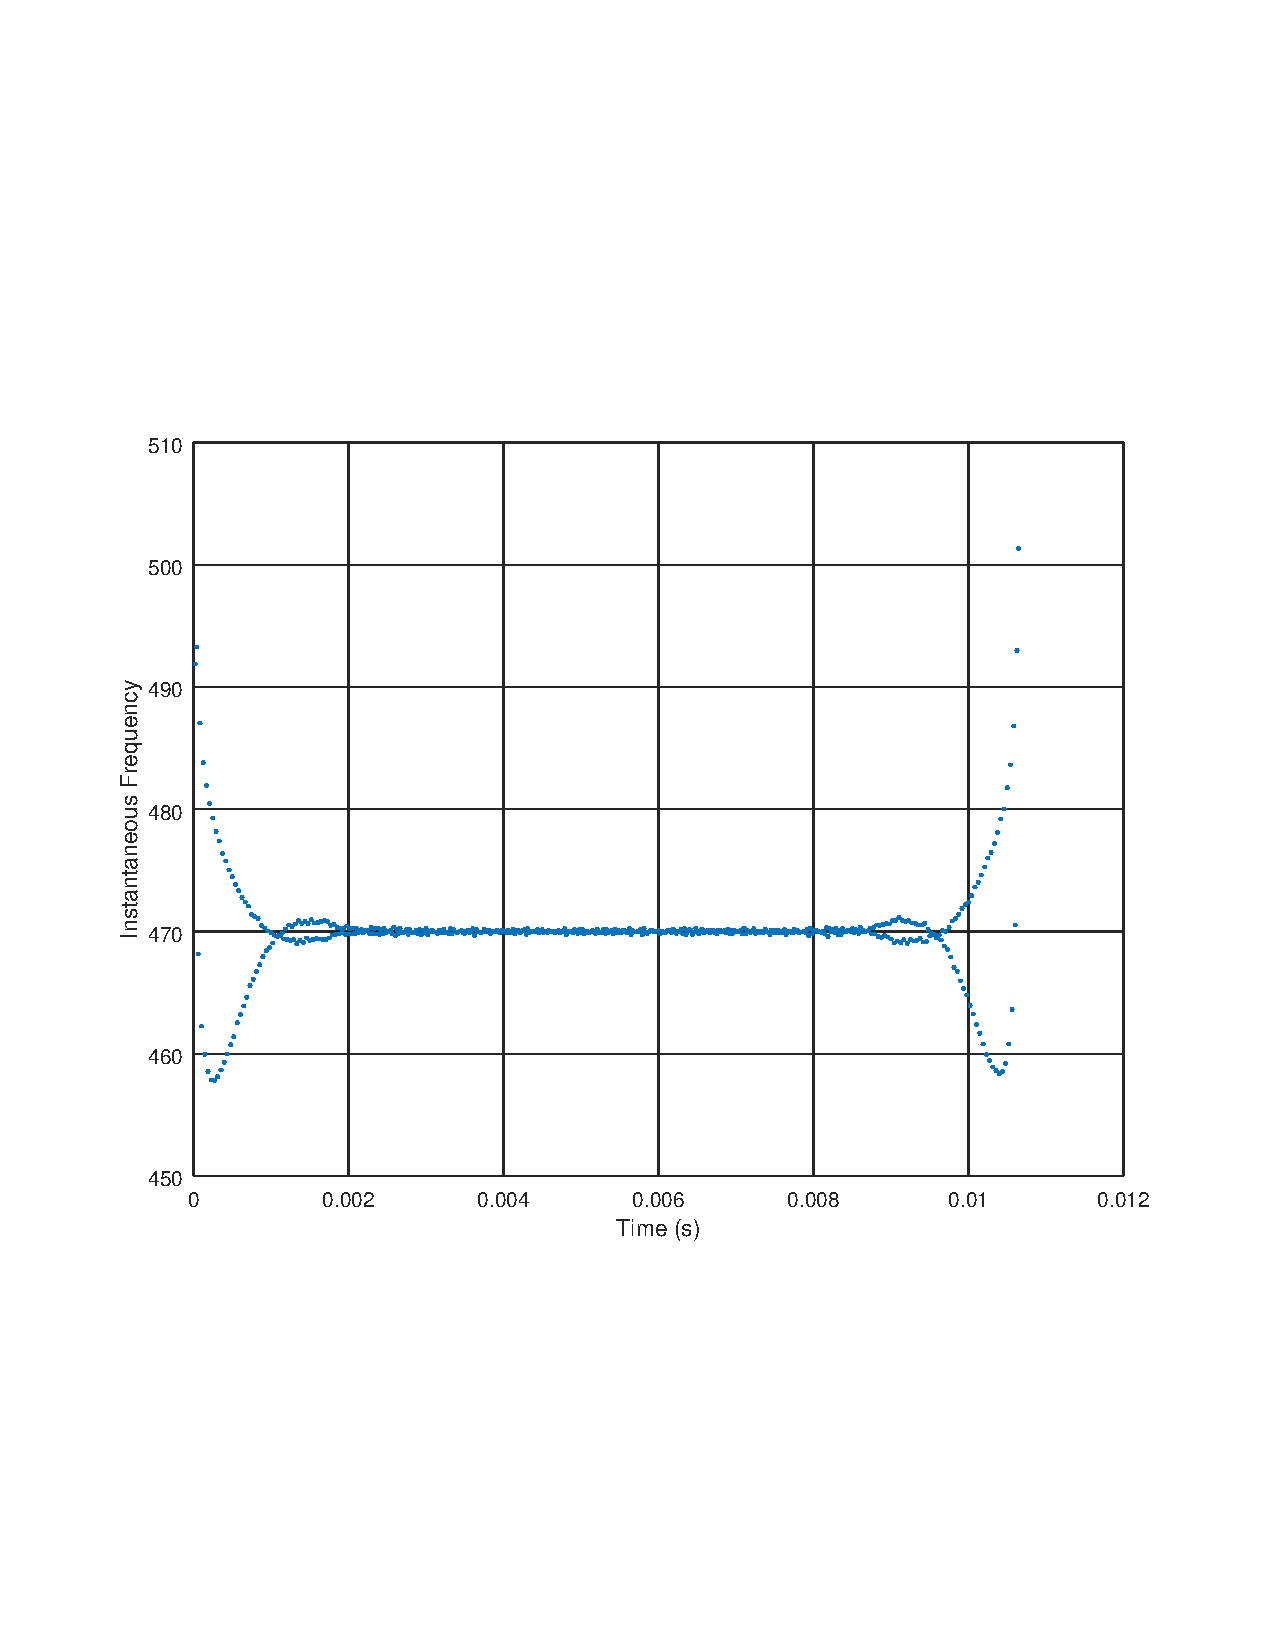
\includegraphics[width=.9\linewidth, clip, trim={2cm 7cm 2cm 7cm}]{gfx/Modelling/IFIF.pdf}
		\caption{Instantaneous Frequency. Derivative of the unwrapped phase.}
		\label{fig:sub3}
	\end{subfigure} 
	\caption{Different steps of determining the Instantaneous Frequency.}
	\label{fig:IFexplained}
\end{figure}

\begin{figure}
	\centering
	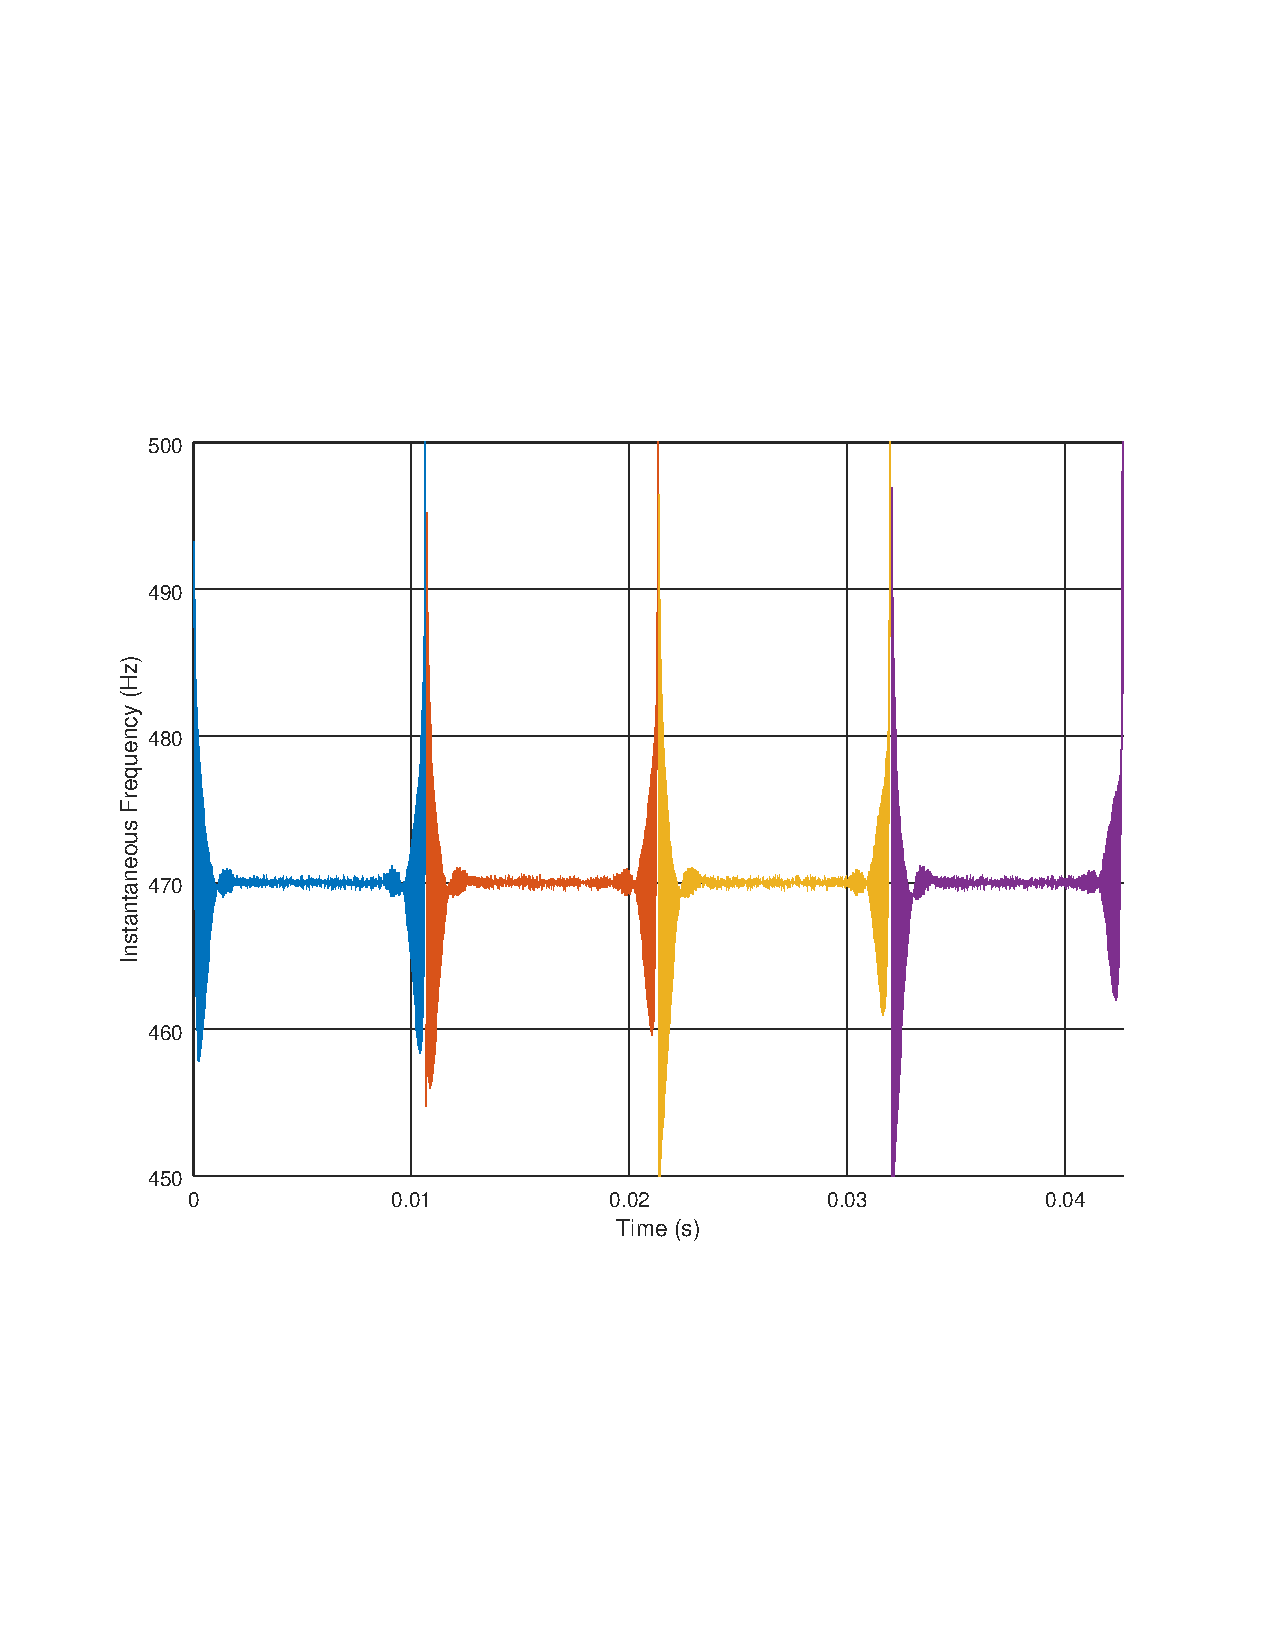
\includegraphics[width=0.7\linewidth, clip, trim={2cm 7cm 2cm 7cm}]{gfx/Modelling/IF.pdf}
	\caption{Instantaneous Frequency, scaled by $\frac{\pi}{2^{15}}$, of the input signal. Each color represents a new block.}
	\label{fig:modelIF}
\end{figure}

\begin{figure}
	\centering
	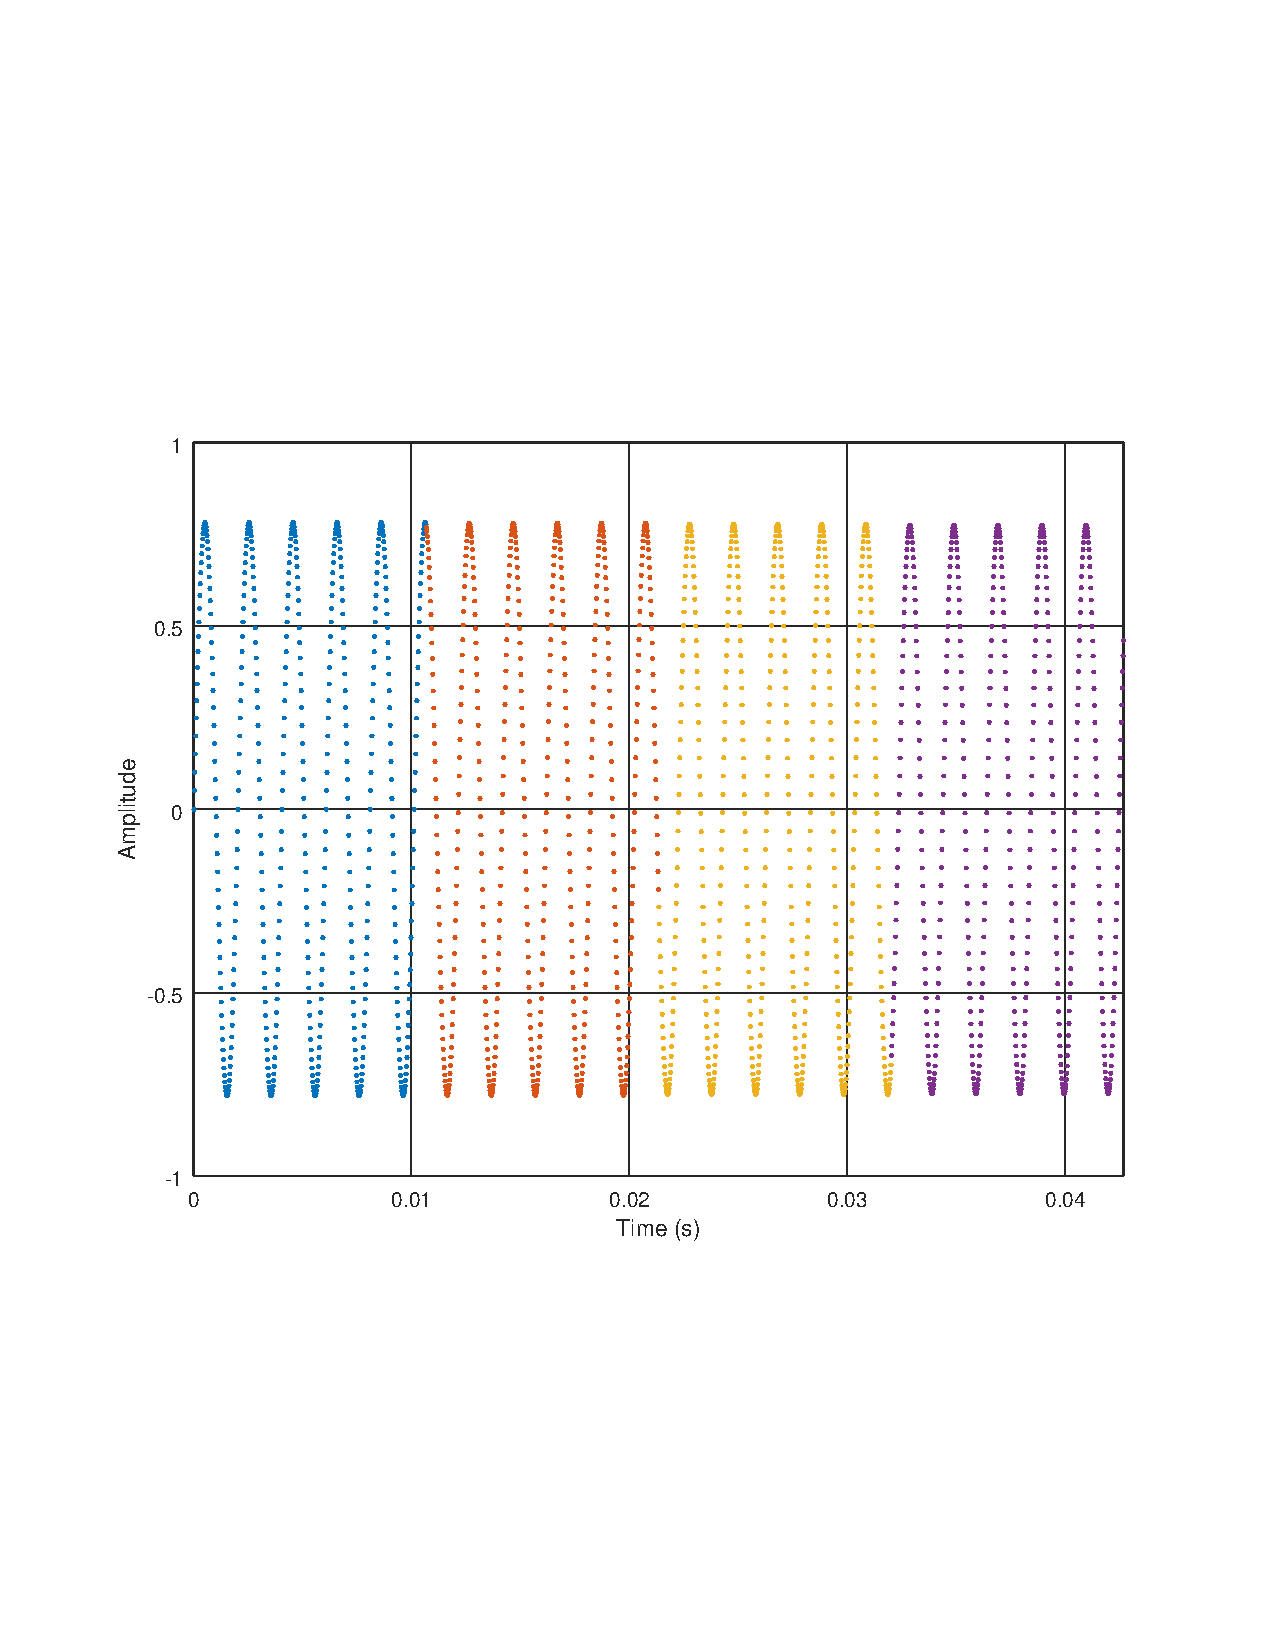
\includegraphics[width=0.7\linewidth, clip, trim={2cm 7cm 2cm 7cm}]{gfx/Modelling/output.pdf}
	\caption{Output signal, scaled by $\frac{1}{2^{15}}$, in the time domain. Each color represents a new block.}
	\label{fig:modelout}
\end{figure}

\FloatBarrier